\begin{frame}{Memorizing}
    Model Predictive Control
    
    The route is given by set of set-points to the leader and the follower receives the set points via a ROS message and calculates by given rules where it should be in that scenario.
    
    
    \section{Planning}
    Planning receives a composite-goal and outputs a set of actions
    
    
    \section{Goal (set-point)}
        A composite goal must be given to the planning that should include:
        
        Keep suprise poise as low as possible in controller cost function.
    
    
    \section{Controller}
        
        Both drones use \textbf{MPC} to reach their next set-point
        
        Feedback system from a feedback that is formed of resource\_gain and goal\_gain
    
    
    \section{Cost function}
        \begin{figure}[H]
            \centering
            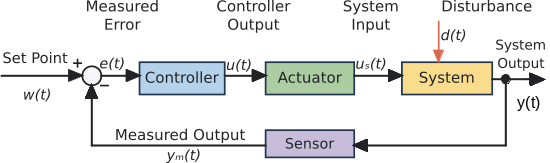
\includegraphics[width=0.9\textwidth]{perception_action_memorizing_loop/a_typical_controller.png}
        \end{figure}
        Both the distances here are measured by Mahalanobis distance
    
    
    \section{Plan}
        
        \textbf{Action}
        
        
        \begin{figure}[H]
            \centering
            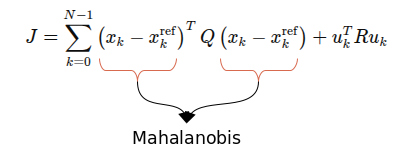
\includegraphics[width=0.9\textwidth]{perception_action_memorizing_loop/mpc_cost_function}
        \end{figure}

\end{frame}